\documentclass[12pt,letterpaper]{article}
\usepackage[margin=1in]{geometry}
\usepackage{fancyhdr}
\usepackage[utf8]{inputenc}
\usepackage{palatino}
\usepackage{microtype}
\usepackage{hyperref}
\usepackage{graphicx}
\usepackage{lastpage}
\usepackage[hang,small,margin=1in]{caption}
\usepackage{titlesec}
\usepackage{pdfpages}

\renewcommand{\headrulewidth}{0pt}
\fancyfoot{}
\fancyfoot[C]{\sffamily Page \thepage\ of \pageref{LastPage}}
\pagestyle{fancy}

\titleformat{\section}{\bfseries\MakeUppercase}{\arabic{\thesection}}{1em}{}
\titleformat{\subsection}{\bfseries}{\arabic{\thesection}.\arabic{\thesubsection}}{1em}{}
\titleformat{\subsubsection}{\itshape}{\arabic{\thesection}.\arabic{\thesubsection}.\arabic{\thesubsubsection}}{1em}{}

\setlength{\parindent}{0cm}
\setlength{\parskip}{1em}

\captionsetup[figure]{labelfont=it, font=it}
\captionsetup[table]{labelfont={it,sc}, font={it,sc}}

\hypersetup{colorlinks, linkcolor = black, citecolor = black, urlcolor = black}
\urlstyle{same}



\begin{document}

\fancyfoot{}
\begin{center}
    \hfill \\
    \vspace{4in}
    {\bf\Huge CS480 Milestone \#2 \\}
    \vspace{2in}
    {\Large Soo-Hyun Yoo \\ January 30, 2015}
\end{center}

\newpage
\fancyfoot[C]{\sffamily Page \thepage\ of \pageref{LastPage}}

% Handwritten answers
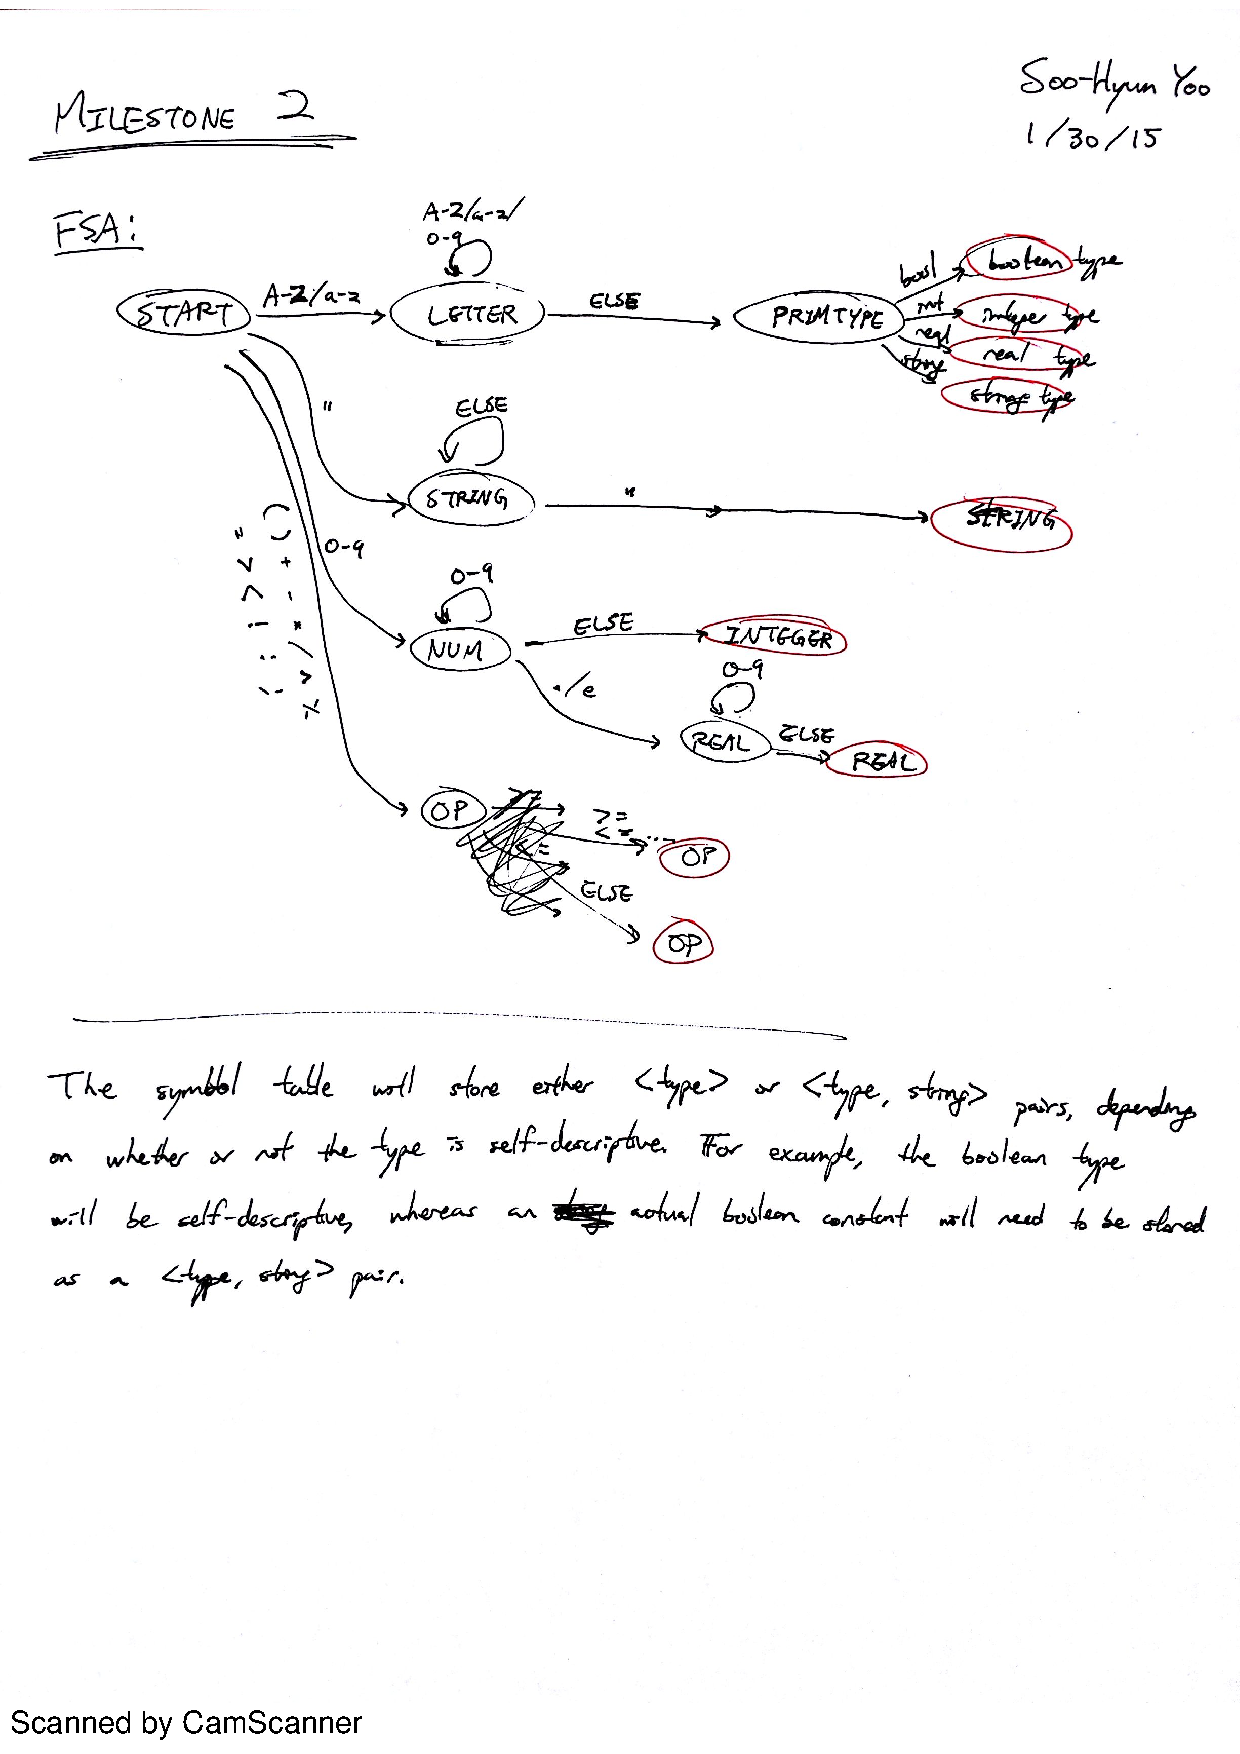
\includepdf[pages={1}]{m2_handwritten.pdf}

\section*{Specification}

This milestone prompts the design and creation of a scanner and symbol table
that will be used to recognize and store IBTL tokens. Importantly, I will learn
to design finite state automata using a state transition diagram before writing
the actual code. Having this consistent model will hopefully preclude headaches
when writing the syntactic and semantic parsers.

\section*{Processing}

All possible token types were identified and categorized. A rough state
transition diagram was constructed to recognize these token types by character.

The state transition graph is composed of several FSAs strung in series with
four initial "top-level" FSAs for lexemes that start with a quotation mark,
letter, number, or special character. These further categorize and accept the
lexemes as actual token types or reject otherwise.

\section*{Testing Requirement}

I tested the lexer for correctness by feeding it as many combinations of token
types as I could reasonably come up with. The lexemes were printed with the
lexer's recognized token type, each of which I checked manually.

\section*{Retrospective}

Code modularity is extremely important in keeping the lexer comprehensible.
This seems to go hand in hand with the consistency of the state transition
model. This also makes it easy to track any special cases (e.g., assign
statement starts with a special character but is not an op).

\end{document}
